% ===== 01-ml-basics =====
\section*{ML Basics \& K-Nearest Neighbors}

\subsection*{Train / Validation / Test Split}
Example: 1000 labeled points $\rightarrow$ 600 train / 200 validation / 200 test.

{\centering
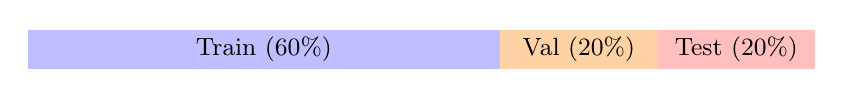
\begin{tikzpicture}
\fill[blue!25]  (0,0) rectangle (6,0.5);  \node[font=\small] at (3,0.25) {Train (60\%)};
\fill[orange!35](6,0) rectangle (8,0.5);  \node[font=\small] at (7,0.25) {Val (20\%)};
\fill[red!25]   (8,0) rectangle (10,0.5); \node[font=\small] at (9,0.25) {Test (20\%)};
\end{tikzpicture}
\par}

\begin{itemize}
  \item \textbf{Train}: the algorithm uses this data to find the best weights $\mathbf{w}$ (e.g.\ the linear regression line).
  \item \textbf{Validation}: we use this data to compare models and pick the best hyperparameters.
  \item \textbf{Test}: we use this data once at the end to see how well the final model does on data it has never seen.
\end{itemize}

\subsection*{K-Nearest Neighbors (KNN)}
\textbf{Idea:} to classify a new point, find the $k$ closest training points and take a majority vote.

{\centering
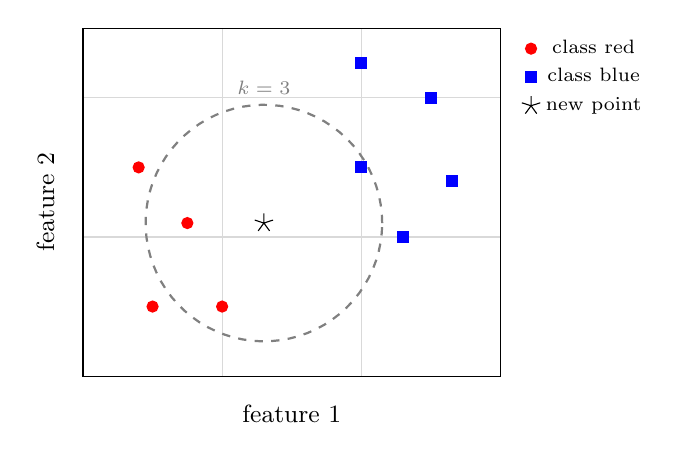
\begin{tikzpicture}
\begin{axis}[
    width=0.6\linewidth, height=6cm,
    xmin=0, xmax=6, ymin=0, ymax=5,
    axis equal image,
    enlargelimits=false, grid=major, grid style={gray!30}, major tick length=0pt,
    xticklabels={}, yticklabels={},
    xlabel={feature 1}, ylabel={feature 2},
    label style={font=\small},
    legend pos=outer north east, legend style={font=\scriptsize, draw=none}
]
\addplot[only marks, mark=*, red, mark size=2pt] coordinates {(1,1) (2,1) (1.5,2.2) (0.8,3)};
\addlegendentry{class red}
\addplot[only marks, mark=square*, blue, mark size=2pt] coordinates {(4,3) (5,4) (4,4.5) (4.6,2) (5.3,2.8)};
\addlegendentry{class blue}
\addplot[only marks, mark=star, black, mark size=3.5pt] coordinates {(2.6,2.2)};
\addlegendentry{new point}
\addplot[dashed, thick, gray, domain=0:360, samples=80, forget plot]
    ({2.6 + 1.7*cos(x)}, {2.2 + 1.7*sin(x)});
\node[font=\scriptsize, anchor=south, gray] at (axis cs:2.6,3.9) {$k=3$};
\end{axis}
\end{tikzpicture}
\par}

\begin{itemize}
  \item The circle holds the 3 nearest neighbors: 2 red and 1 blue, so the new point is predicted \textbf{red}.
  \item Change $k$ and the answer can change. A bigger circle may pull in more blue points.
  \item \textbf{Confidence} = the share of neighbors that voted for the winning class (here, 2 out of 3).
  \item \textbf{No training step}: KNN just stores the data. Prediction is the slow part, because it measures the distance to every training point.
  \item \textbf{Standardize features first.} Otherwise the feature with the biggest units (e.g.\ pounds vs.\ inches) dominates the distance.
\end{itemize}

\subsection*{Overfitting vs.\ Underfitting}

\textbf{Example.} Fit three models of increasing flexibility to the same 8 noisy training points (blue):

{\centering
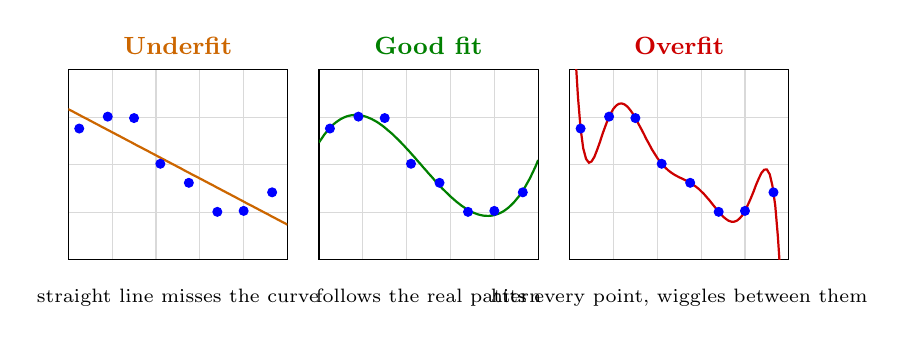
\begin{tikzpicture}
\begin{axis}[name=p0,
    width=0.36\linewidth, height=4cm,
    xmin=0, xmax=1, ymin=-2, ymax=2, enlargelimits=false,
    grid=major, grid style={gray!30}, major tick length=0pt,
    xticklabels={}, yticklabels={},
    title={\small\textbf{Underfit}}, title style={text=orange!80!black, yshift=-4pt},
    xlabel={\scriptsize straight line misses the curve}, label style={font=\scriptsize}]
\addplot[only marks, mark=*, blue, mark size=1.6pt] coordinates {(0.05,0.76) (0.18,1.01) (0.3,0.98) (0.42,0.02) (0.55,-0.38) (0.68,-0.99) (0.8,-0.97) (0.93,-0.58)};
\addplot[thick, orange!80!black] coordinates {(0.000,1.167) (0.013,1.137) (0.025,1.107) (0.038,1.076) (0.050,1.046) (0.062,1.016) (0.075,0.985) (0.088,0.955) (0.100,0.925) (0.113,0.894) (0.125,0.864) (0.138,0.834) (0.150,0.803) (0.163,0.773) (0.175,0.743) (0.188,0.712) (0.200,0.682) (0.213,0.652) (0.225,0.621) (0.238,0.591) (0.250,0.561) (0.263,0.530) (0.275,0.500) (0.288,0.470) (0.300,0.439) (0.312,0.409) (0.325,0.379) (0.338,0.348) (0.350,0.318) (0.363,0.288) (0.375,0.257) (0.388,0.227) (0.400,0.197) (0.413,0.166) (0.425,0.136) (0.438,0.106) (0.450,0.075) (0.463,0.045) (0.475,0.015) (0.488,-0.016) (0.500,-0.046) (0.513,-0.076) (0.525,-0.107) (0.537,-0.137) (0.550,-0.167) (0.562,-0.198) (0.575,-0.228) (0.588,-0.258) (0.600,-0.289) (0.613,-0.319) (0.625,-0.349) (0.638,-0.380) (0.650,-0.410) (0.663,-0.440) (0.675,-0.471) (0.688,-0.501) (0.700,-0.531) (0.713,-0.562) (0.725,-0.592) (0.738,-0.622) (0.750,-0.653) (0.763,-0.683) (0.775,-0.714) (0.788,-0.744) (0.800,-0.774) (0.812,-0.805) (0.825,-0.835) (0.838,-0.865) (0.850,-0.896) (0.863,-0.926) (0.875,-0.956) (0.888,-0.987) (0.900,-1.017) (0.913,-1.047) (0.925,-1.078) (0.938,-1.108) (0.950,-1.138) (0.963,-1.169) (0.975,-1.199) (0.988,-1.229) (1.000,-1.260)};
\end{axis}
\begin{axis}[name=p1, at={(p0.east)}, anchor=west, xshift=0.4cm,
    width=0.36\linewidth, height=4cm,
    xmin=0, xmax=1, ymin=-2, ymax=2, enlargelimits=false,
    grid=major, grid style={gray!30}, major tick length=0pt,
    xticklabels={}, yticklabels={},
    title={\small\textbf{Good fit}}, title style={text=green!50!black, yshift=-4pt},
    xlabel={\scriptsize follows the real pattern}, label style={font=\scriptsize}]
\addplot[only marks, mark=*, blue, mark size=1.6pt] coordinates {(0.05,0.76) (0.18,1.01) (0.3,0.98) (0.42,0.02) (0.55,-0.38) (0.68,-0.99) (0.8,-0.97) (0.93,-0.58)};
\addplot[thick, green!50!black] coordinates {(0.000,0.466) (0.013,0.555) (0.025,0.636) (0.038,0.709) (0.050,0.774) (0.062,0.832) (0.075,0.882) (0.088,0.925) (0.100,0.961) (0.113,0.990) (0.125,1.013) (0.138,1.030) (0.150,1.040) (0.163,1.045) (0.175,1.045) (0.188,1.038) (0.200,1.027) (0.213,1.011) (0.225,0.990) (0.238,0.965) (0.250,0.936) (0.263,0.903) (0.275,0.866) (0.288,0.825) (0.300,0.781) (0.312,0.734) (0.325,0.684) (0.338,0.632) (0.350,0.577) (0.363,0.520) (0.375,0.462) (0.388,0.401) (0.400,0.339) (0.413,0.276) (0.425,0.212) (0.438,0.147) (0.450,0.081) (0.463,0.015) (0.475,-0.051) (0.488,-0.117) (0.500,-0.182) (0.513,-0.247) (0.525,-0.311) (0.537,-0.375) (0.550,-0.436) (0.562,-0.497) (0.575,-0.555) (0.588,-0.612) (0.600,-0.667) (0.613,-0.719) (0.625,-0.768) (0.638,-0.815) (0.650,-0.859) (0.663,-0.899) (0.675,-0.936) (0.688,-0.969) (0.700,-0.998) (0.713,-1.022) (0.725,-1.043) (0.738,-1.058) (0.750,-1.069) (0.763,-1.074) (0.775,-1.075) (0.788,-1.069) (0.800,-1.058) (0.812,-1.041) (0.825,-1.018) (0.838,-0.988) (0.850,-0.951) (0.863,-0.907) (0.875,-0.856) (0.888,-0.798) (0.900,-0.732) (0.913,-0.659) (0.925,-0.577) (0.938,-0.487) (0.950,-0.388) (0.963,-0.281) (0.975,-0.164) (0.988,-0.038) (1.000,0.097)};
\end{axis}
\begin{axis}[name=p2, at={(p1.east)}, anchor=west, xshift=0.4cm,
    width=0.36\linewidth, height=4cm,
    xmin=0, xmax=1, ymin=-2, ymax=2, enlargelimits=false,
    grid=major, grid style={gray!30}, major tick length=0pt,
    xticklabels={}, yticklabels={},
    title={\small\textbf{Overfit}}, title style={text=red!80!black, yshift=-4pt},
    xlabel={\scriptsize hits every point, wiggles between them}, label style={font=\scriptsize}]
\addplot[only marks, mark=*, blue, mark size=1.6pt] coordinates {(0.05,0.76) (0.18,1.01) (0.3,0.98) (0.42,0.02) (0.55,-0.38) (0.68,-0.99) (0.8,-0.97) (0.93,-0.58)};
\addplot[thick, red!80!black] coordinates {(0.000,2.400) (0.013,2.400) (0.025,2.396) (0.038,1.422) (0.050,0.760) (0.062,0.345) (0.075,0.121) (0.088,0.042) (0.100,0.068) (0.113,0.166) (0.125,0.308) (0.138,0.474) (0.150,0.646) (0.163,0.810) (0.175,0.957) (0.188,1.081) (0.200,1.177) (0.213,1.244) (0.225,1.280) (0.238,1.287) (0.250,1.267) (0.263,1.223) (0.275,1.158) (0.288,1.075) (0.300,0.980) (0.312,0.875) (0.325,0.765) (0.338,0.652) (0.350,0.539) (0.363,0.430) (0.375,0.326) (0.388,0.230) (0.400,0.142) (0.413,0.063) (0.425,-0.007) (0.438,-0.067) (0.450,-0.119) (0.463,-0.164) (0.475,-0.202) (0.488,-0.235) (0.500,-0.264) (0.513,-0.292) (0.525,-0.319) (0.537,-0.348) (0.550,-0.380) (0.562,-0.416) (0.575,-0.457) (0.588,-0.504) (0.600,-0.557) (0.613,-0.616) (0.625,-0.680) (0.638,-0.748) (0.650,-0.819) (0.663,-0.892) (0.675,-0.963) (0.688,-1.029) (0.700,-1.089) (0.713,-1.139) (0.725,-1.176) (0.738,-1.196) (0.750,-1.197) (0.763,-1.176) (0.775,-1.131) (0.788,-1.063) (0.800,-0.970) (0.812,-0.855) (0.825,-0.722) (0.838,-0.577) (0.850,-0.429) (0.863,-0.289) (0.875,-0.174) (0.888,-0.103) (0.900,-0.102) (0.913,-0.202) (0.925,-0.438) (0.938,-0.855) (0.950,-1.504) (0.963,-2.400) (0.975,-2.400) (0.988,-2.400) (1.000,-2.400)};
\end{axis}
\end{tikzpicture}
\par}

\begin{keeptogether}
\begin{itemize}
  \item \textbf{Underfit}: too simple to capture the pattern, so it is wrong on training \emph{and} new data.
  \item \textbf{Overfit}: it memorized the noise. Training error is 0, but new points between the dots get predicted badly.
  \item \textbf{Good fit}: misses each point a little, but predicts new points well.
\end{itemize}

\begin{center}
\begin{tabular}{lccl}
\toprule
 & Train error & Validation error & Cause \\
\midrule
Underfit & high & high & model too simple (high bias) \\
Good fit & low & low & captures the pattern, not the noise \\
Overfit & very low & high & memorizes noise (high variance) \\
\bottomrule
\end{tabular}
\end{center}
\end{keeptogether}

\subsection*{Bias vs.\ Variance}
% TODO
